%!TEX root = ../../main.tex
\section{Radiation damage in MX}
\label{sec:Radiation damage in MX}
    A common theme amongst all of the structural techniques mentioned thus far is that the sample is probed with ionising radiation.
    This results in the sample suffering radiation damage (even samples studied at XFEL sources also show signs of radiation damage with a long enough pulse \cite{nass2015indications}).
    Being the most mature of these structural techniques however, much more literature exists about radiation damage for synchrotron based MX.
    Radiation damage is a problem because limits the amount of useful data that can be collected from a single crystal during an MX experiment \cite{garman2010}.
    It is therefore the major cause of unsuccessful data collection at synchrotron sources given a sufficiently diffracting crystal \cite{zeldin2013dwd}.

    \subsection{Types of X-ray interactions with atoms: Primary damage}
    \label{sub:Types of X-ray interactions with atoms: Primary damage}
        In a fairly typical MX experimental set-up only a small fraction of the incident X-ray photons will interact in any way with the atoms in the crystal. Garman reported that for a $100\ \mu m$ thick protein crystal only 2\% of the incident photons of a $12.4\ keV$ (1\ \AA) incident beam with interact with it \cite{garman2010}.
        This section will explain the possible interactions that occur and how they can give rise to the data or result in radiation damage

        \subsubsection{Elastic scattering}
        \label{subs:Elastic scattering}
            Elastic scattering (also referred to as Rayleigh, Thompson or coherent scattering) is a type of interaction in which no energy from the incident X-ray photon is deposited in the sample \cite{nave1995}.
            The resulting scattered waves interfere to give rise to the observed diffraction pattern.
            It is the type of interaction that the experimenter would like to maximise. However, of the 2\% of the incident X-ray photons that interact with the sample, only about 8\% of that results in elastic scattering \cite{ravelli2006radiation}.

        \subsubsection{Compton Scattering}
        \label{subs:Compton Scattering}
            Another 8\% of the interaction is due to Compton scattering. This type of scattering occurs when the X-ray photon scatters incoherently from the crystal, thereby transferring some of its energy to an electron.
            The resulting scattered X-ray photon leaves with less energy (higher wavelength). It is possible for the recoil electron (the name given to the electron in which the energy is deposited) to also be ejected from the atom \cite{nave1995}.

        \subsubsection{Photoelectric effect}
        \label{subs:Photoelectric effect}
            By far the most common interaction is the photoelectric effect which is responsible for the other 84\% of the X-ray-electron interactions.
            In this type of interaction, the incident X-ray photon is completely absorbed and an inner shell electron is ejected \cite{garman2010}.
            The ejected electron is called a photoelectron. The vacancy left by the ejection of the photoelectron is filled by another electron.
            This transition can lead to two different outcomes: either the production of a characteristic X-ray, known as fluorescence, or the ejection of an electron from an outer shell \cite{nave1995}.
            The ejected electron is known as the Auger electron. The relative probability of either fluorescence or Auger emission occurring is dependent on the atomic species.
            With lighter elements that constitute the vast majority of protein molecules the more likely process is Auger emission.

        An ionisation event caused by the photoelectric effect or Compton scattering is referred to as primary damage, although the use of this term varies in the literature \cite{garman2010}.
        The relative probability of each of the three interactions (cross section) described above varies with incident X-ray beam energy (Figure~\ref{fig:Relative Absorption Probabilities}). The atomic number also affects the amount of energy absorption in the sample with heavier elements contributing more to the overall absorption per atom.
        To maximise the amount of elastic scattering it would initially seem advisable to increase the energy of the incident X-ray beam from the range of typical values used in X-ray crystallography, usually around $12\ keV$ \cite{pait2010}.
        However, the diffracted intensity per incident photon is lower for incident beams with higher energy. In practice, the optimal energy for an MX experiment is highly dependent on the sample composition and the aims of the experiment (i.e. the design may be different if the experiment aims to collect suitable data for phasing) and no general consensus has been established \cite{pait2010}.
        \begin{figure}
            \centering
            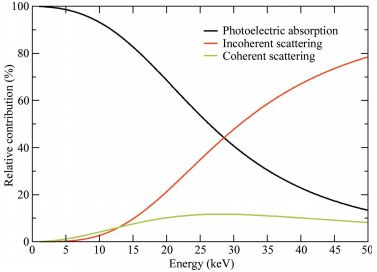
\includegraphics[width=0.6\textwidth]{figures/introduction/relativeinteractions.png}
            \caption{Relative contribution to the overall X-ray cross section as a function of incident beam energy for chicken egg-white lysozyme \cite{pait2010}. The photoelectric effect dominates the interaction cross section at typical wavelengths used in MX (about $12\ keV$). However, at higher energies the elastic contribution increases but the Compton effect increases faster and begins to dominate.}
            \label{fig:Relative Absorption Probabilities}
        \end{figure}

    \subsection{Secondary damage}
    \label{sub:Secondary damage}
        In contrast to primary damage (ionisation due to the incident photon), secondary damage is the damage caused by the energetic electrons produced as a result of the former.
        In fact it is secondary damage that is responsible for the majority of the damage that is observed in MX experiments.
        A single photoelectron has enough energy to cause $\approx$ 500 ionisation events \cite{o2002physical}. The ionisation event is referred to as direct damage if the event occurs within the protein molecule.
        If the event occurs within the surrounding mother liquor then it is referred to as indirect damage.
        The radical species produced as a result of these events can diffuse through the crystal disrupting the structure of the proteins by breaking chemical bonds, causing redox processes and producing more radical species \cite{meents2010}.
		Some of the radical species produced are hydroxyl radicals, electrons and hydrogen ions \cite{garman2010}.
        At temperatures below $\approx 180\ K$ (the glass transition) it is thought that the only mobile radical species are electrons \cite{jones1987structure} due to the solvent possessing a quasi-infinite viscosity \cite{weik2001specific}.
		Electrons are able to overcome energy barriers by quantum mechanical tunnelling mechanisms \cite{garman2009radiation} and cause the majority of the damage observed in MX experiments \cite{garman2010}.

    \subsection{Quantifying energy absorbance: Dose}
    \label{sub:Quantifying energy absorbance: Dose}
        Being able to quantify the amount of energy absorbed by the crystal is vital to track the progression of radiation damage in an MX experiment \cite{blake1962,holton2009}.
        Dose is the metric by which the energy absorbed in the crystal is quantified. The dose is defined as the energy absorbed per unit mass and the SI unit used in MX is the gray ($Gy$), where $1\ Gy = 1\ J\ kg^{-1}$.
        In typical cryo-MX experiments it is common for a crystal to receive a dose that ranges in the order of millions of gray ($MGy$) \cite{garman2010} due to the brilliance of third generation synchrotron sources \cite{mitchell1999}.
        However, due to the complex processes (e.g. the stochastic nature of the absorption events, electron cascades, etc.), direct measurement of the dose is infeasible and so it must be calculated instead.
        The formula used to calculate the dose for a small volume of sample is
        \begin{equation}
            Dose = \f{E_{incident}}{M_{vol}} \left(1- e^{-\mu_{abs}z}\right),
            \label{eq:Dose Calculation 1D}
        \end{equation}
        Where $E_{incident}$ is the energy incident on the sample, $M_{vol}$ is the mass of the irradiated volume and $1- e^{-\mu_{abs}z}$ is the fraction of the incident beam absorbed through the volume of thickness $z$, $\mu_{abs}$ is the absorption coefficient of the sample (a value dependent on the atomic cross sections that determines the likelihood of absorbance of the X-ray beam) and $e = 2.718 \ldots$ is Euler's number \cite{zeldin2013thesis}.

        RADDOSE is a software program that was developed to improve the ease of calculating the absorbed dose within a protein crystal \cite{murray2004}. It increases the accuracy by implementing a 2D model of the experiment as opposed to the 1D model in equation \ref{eq:Dose Calculation 1D}.
        Information about the crystal (size, unit cell parameters, number of molecules per unit cell, number of residues, solvent content), the beam (energy, flux, and profile), exposure time per image and the total number of images is required for the calculation.
        RADDOSE uses these parameters to determine the maximum beam intensity and simulates an experiment by which the crystal is exposed homogeneously to the beam to provide a worst case scenario dose estimate: the maximum dose.
        Several improvements to the model were incorporated in successive versions of RADDOSE.
        Version two \cite{pait2009} calculated the fluorescent emission probability and the probability that these fluorescent photons could escape the crystal.
        Version three \cite{pait2010} took into account energy loss in the crystal due to the Compton Effect.

        Despite these improvements RADDOSE has several drawbacks. One of the major problems with the dose calculation is that some parameters of the data collection experiment are known with more certainty than others.
        Parameters such as the crystal composition, beam flux and exposure time are known to a relatively high degree of accuracy.
        However, the extent to which parameters such as the crystal volume \cite{holton2009} and beam profile \cite{krojer2011} are known can be significantly less.
        This can lead to large errors in the calculated dose values and inferences about the radiation susceptibility of protein crystals \cite{krojer2011}.
        The uncertainty can be accounted for by assigning a ``factor of 2" decision threshold \cite{holton2009}.
		This means that a particular radiation damage effect described by quantitative values (e.g. intensity loss or dose) can be considered the same if the values are within a factor of 2 of each other.
        Methods are being developed to better parametrise the data collection experiment for the crystal shape \cite{svensson2015fully,khan2012confocal,brockhauser2008x} and the beam \cite{bowler2015massif} but these methods are not routine on the majority of beamlines.

        Another problem encountered with the calculation of dose in RADDOSE is the two-dimensional nature of the model. It means that it lacks the three-dimensional information about the damage state of the crystal.
        This information is important for optimising the use of crystal volume to collect better quality data \cite{zeldin2012,zeldin2013dwd}.
        Furthermore it assumes that the crystal is always immersed within the beam and does not take into account crystal rotation.

        The geometric issues are addressed in the RADDOSE-3D \cite{zeldin2013} software program, a successor to RADDOSE.
        RADDOSE-3D takes into account the three-dimensional geometry of the MX experiment to provide a temporally and spatially resolved dose distribution within a protein crystal.
        Initially RADDOSE-3D was written to model cuboid or spherical crystals, but now it has been extended to be able to capture any polyhedron (Figure~\ref{fig:RADDOSE-3D Polyhedral Crystal Examples}).

        \begin{figure}
            \centering
            \begin{subfigure}[b]{0.463\textwidth}
                    \centering
                    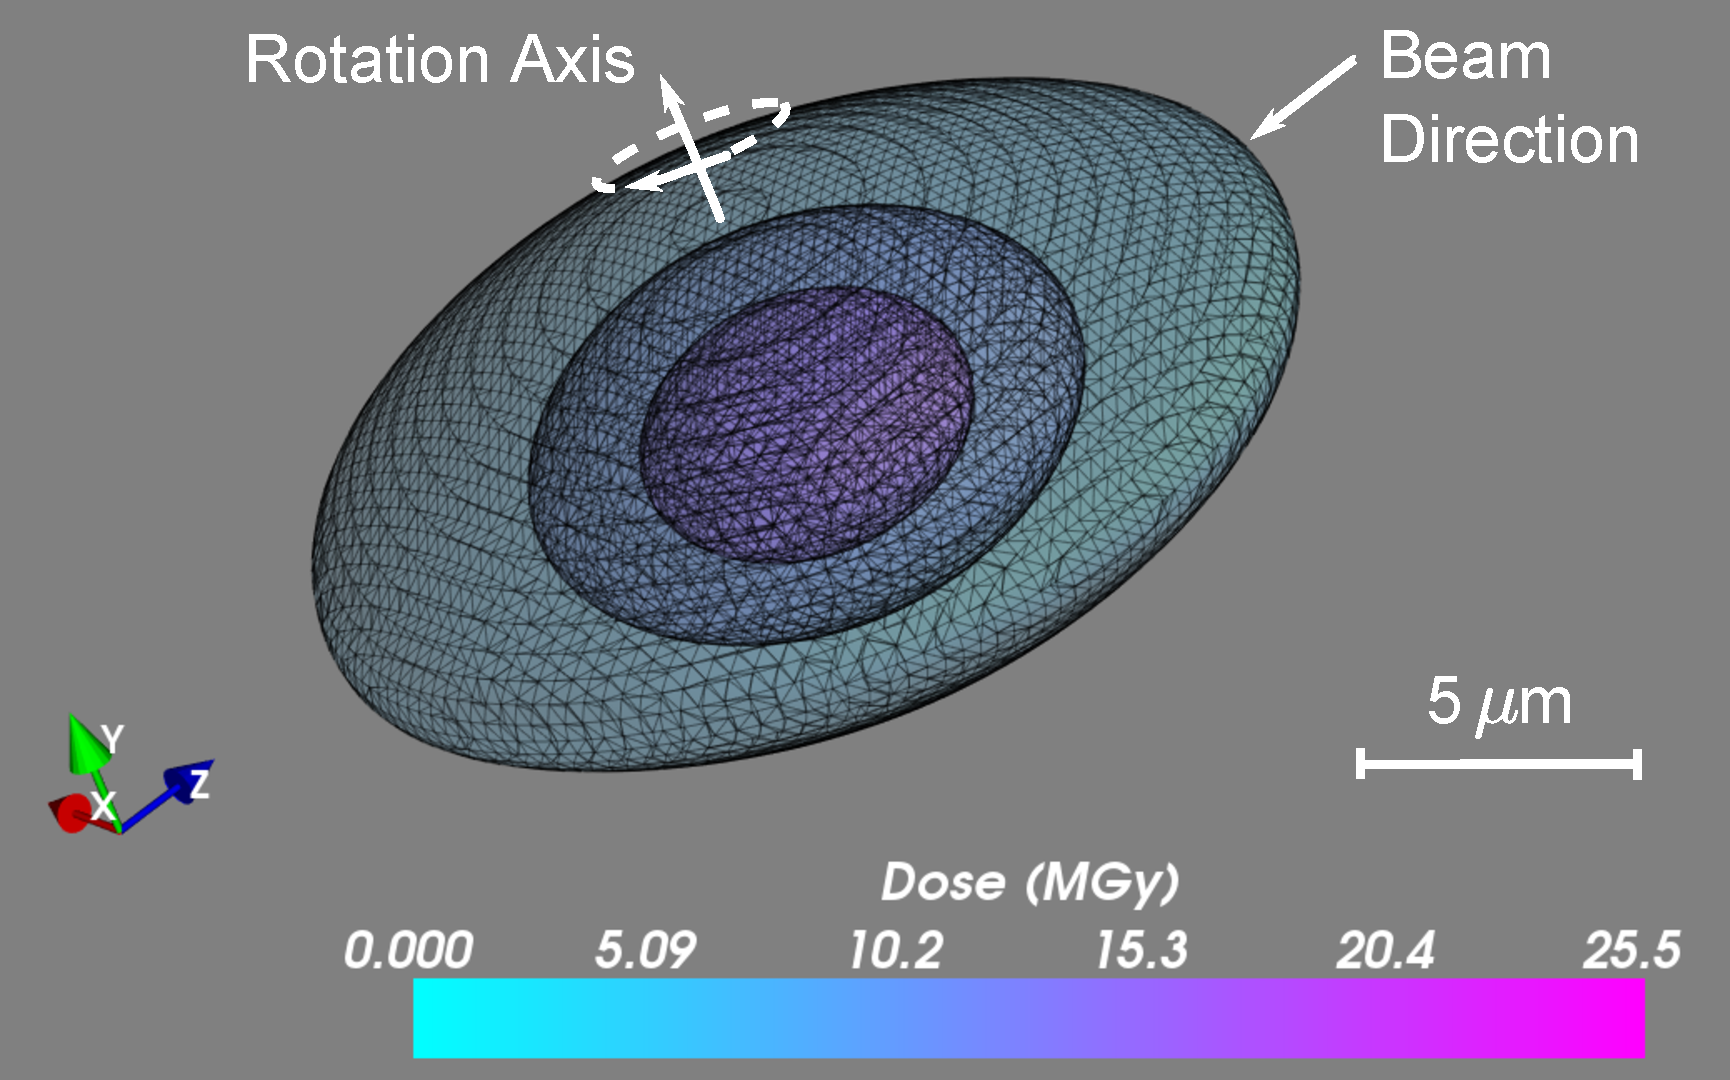
\includegraphics[width=\textwidth]{figures/introduction/ellipsoidcrystal.pdf}
                    \caption{}
                    \label{fig:Ellipsoidal crystal}
            \end{subfigure}
            \quad
            \begin{subfigure}[b]{0.437\textwidth}
                    \centering
                    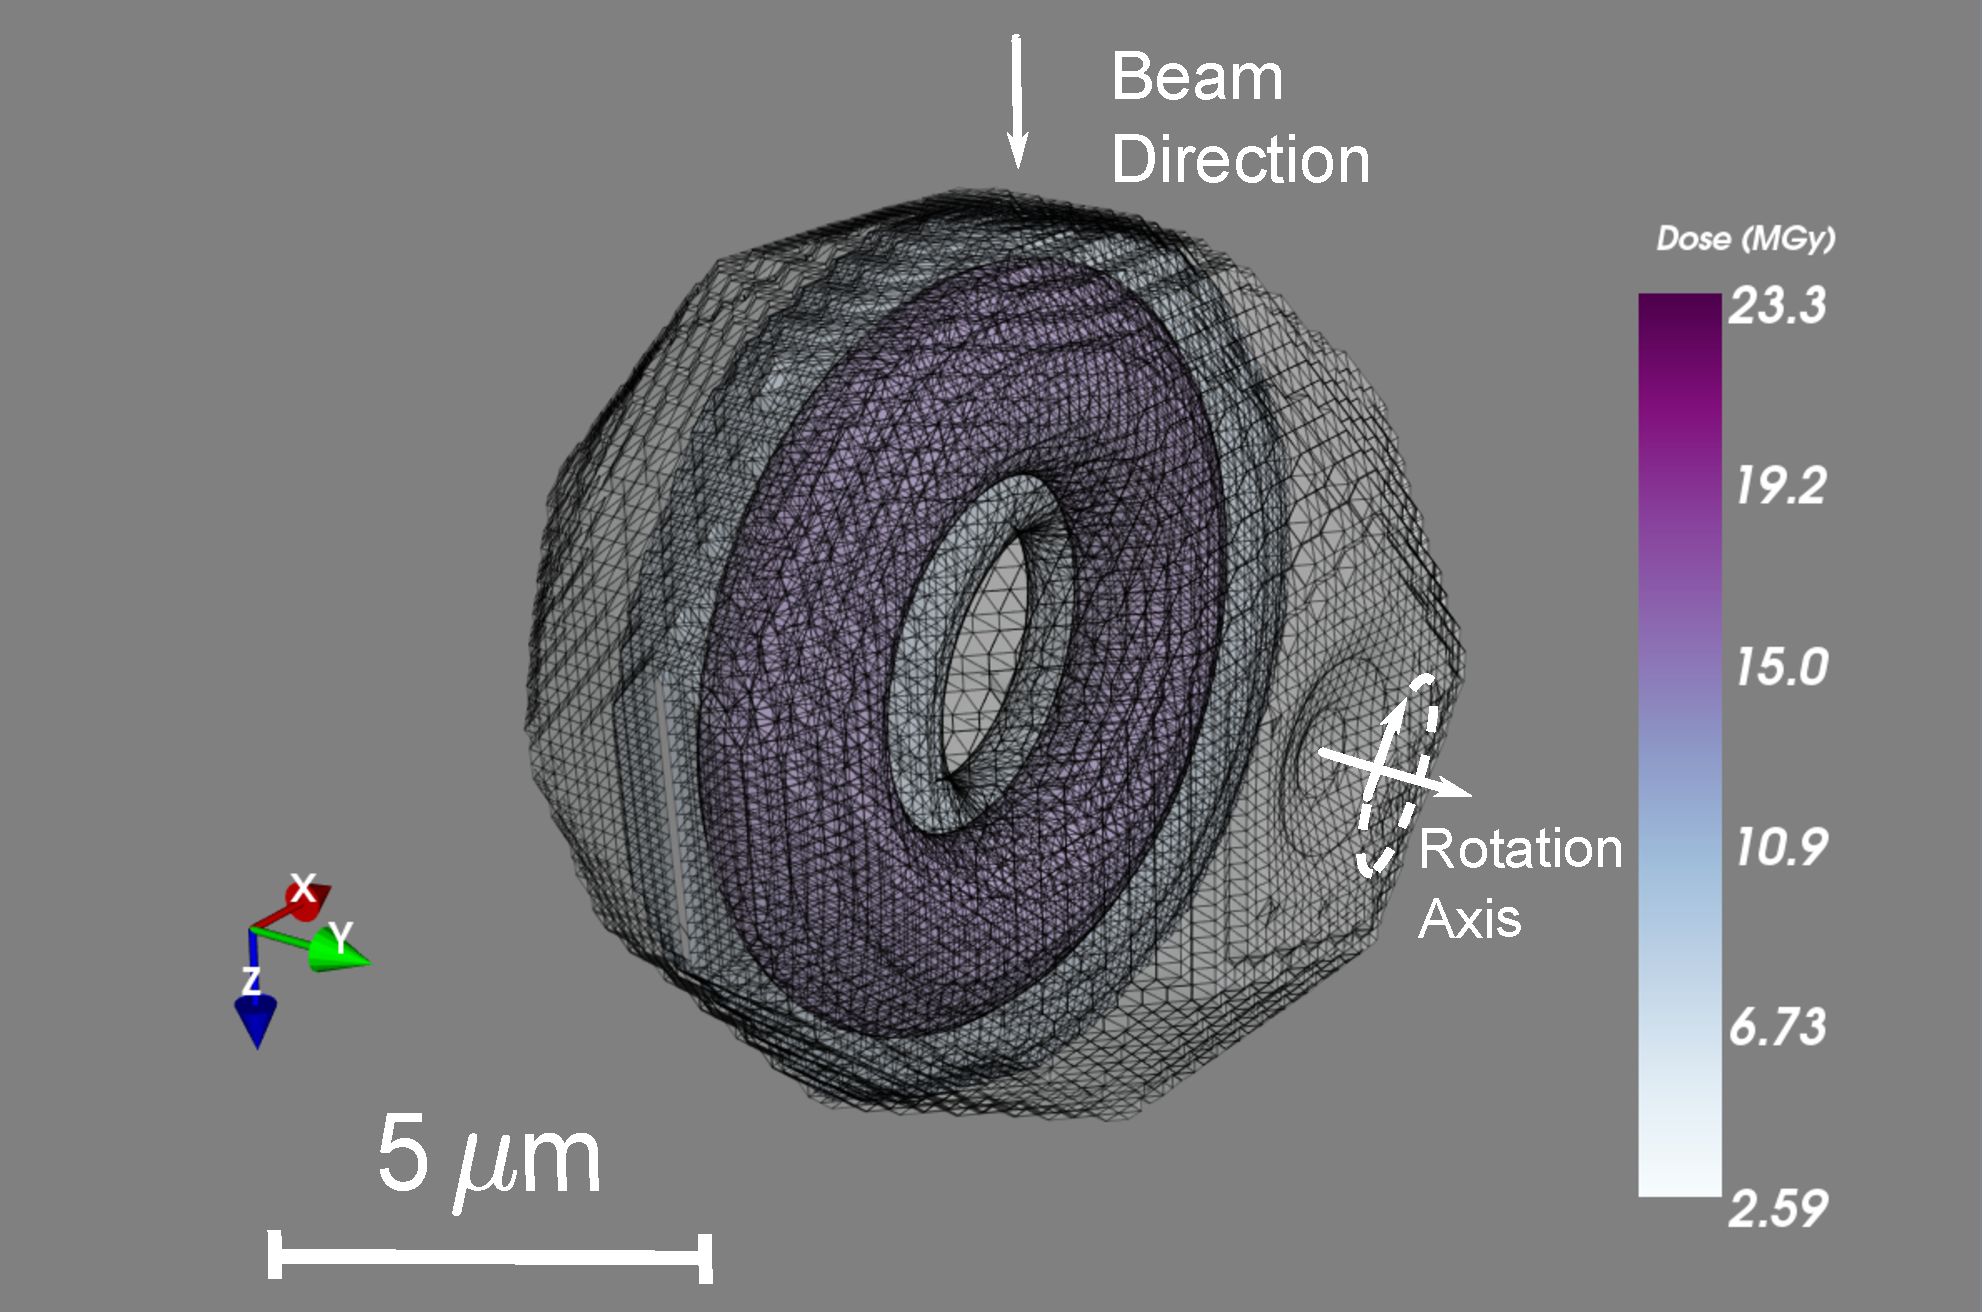
\includegraphics[width=\textwidth]{figures/introduction/IcoCrystalEdges.pdf}
                    \caption{}
                    \label{fig:Icosohedral crystal}
            \end{subfigure}
            \caption{Dose distributions in crystals represented as a polyhedron. (a) An oblate ellipsoid ($x = z = 10\ \mu m$, $y = 6\ \mu m$) crystal that has been irradiated with a Gaussian profile beam with a full width half maximum (FWHM) of $5\ \mu m \times 5\ \mu m$, flux of $10^{10}$ photons per second and an incident photon energy of $12.7 keV$ for a rotation of $360^{\circ}$.
            The collimation was set to $20\ \mu m \times 20\ \mu m$ and hence the entire volume of the crystal was irradiated. The 3 visible contours represent dose values of $20\ MGy, 15\ MGy$ and $5\ MGy$ from inner to outer contour levels.
            (b) An icosahedral crystal with maximum dimensions of $10\ \mu m$ in each of the $x, y$ and $z$ dimensions, which has been irradiated with a Gaussian profile beam with FWHM $4\ \mu m$ in both the $z$ and $y$ directions, flux $2 \times 10^{10}$ photons per second and an incident photon energy of $12.7\ keV$. The rotation axis was offset $5\ \mu m$ from the centre of the crystal in the $x$-direction and the crystal was rotated $360^{\circ}$ for a total exposure time of 180 seconds. Contouring levels correspond to $2.59\ MGy$, $12.5\ MGy$ and $18.75\ MGy$ from inner to outer contour levels. It is evident that different crystal, beam and experiment design parameters lead to very different distributions of absorbed dose within a protein crystal.}
            \label{fig:RADDOSE-3D Polyhedral Crystal Examples}
        \end{figure}

        The raw output of RADDOSE-3D is a 3D scalar field which assigns a dose to every voxel (3D volume element) in the crystal.
        In its raw form, these data are not very useful for the experimenter to assess the damage state of the crystal, especially when the dose distributions are highly inhomogeneous (Figure~\ref{fig:RADDOSE-3D Polyhedral Crystal Examples}).
        So several metrics were proposed to provide useful summaries of the data.
        These include the maximum dose (the same dose value as output by the original versions of RADDOSE), average dose for the whole crystal and the dose inefficiency (i.e. the maximum dose divided by the absorbed energy), amongst others \cite{zeldin2012}.
        The metric that was found to be most promising in faithfully representing the damage state of the crystal is the diffraction weighted dose (DWD) \cite{zeldin2013dwd}. The DWD is a weighted average, where the weight at each voxel position in the crystal is given by the X-ray fluence through that voxel.
        It considers the effective dose absorbed by the crystal and its impact on the diffraction pattern for any given image of the dataset. Mathematically the DWD is defined for each image as
        \begin{equation}
            DWD^i = \f{\int_{t_{i-1}}^{t_i} \int_{crystal} D(\bs{x},t) \times F(\bs{x},t)\ \mathrm{d}\bs{x}\mathrm{d}t}{\int_{t_{i-1}}^{t_i} \int_{crystal} F(\bs{x},t)\ \mathrm{d}\bs{x}\mathrm{d}t}
        \end{equation}
        where $i$ is the image number, $t$ is the time, $\bs{x}$ is the position in the crystal, $D$ is the total cumulative absorbed dose ($Gy$) at that position, and $F$ is the fluence (photons per unit area).

        The DWD metric only takes into account the fluence incident on a unit volume during the collection of data for a given image, but does not take into account the loss of diffraction efficiency of the volume due to global radiation damage.
        As the dose increases, a particular volume of the crystal will only contribute to the background \cite{blake1962}.

    \subsection{Manifestations of damage: Global damage}
    \label{sub:Manifestations of damage: Global damage}
        The damage processes described in sections \ref{sub:Types of X-ray interactions with atoms: Primary damage} and \ref{sub:Secondary damage} are observed in a variety of ways in MX which are classified accordingly.
        Global radiation damage is observed in reciprocal space and results in changes in mosaicity, increase in the scaling and atomic $B$ factors, unit cell expansion, increases in data quality $R$ values ($R_{merge}, R_{meas}, R_{pim}$) and decreasing $CC_{1/2}$ and $CC^*$ \cite{garman2010}.
        Perhaps the most iconic symptom of global radiation damage is the loss of intensity of reflections in the diffraction pattern, with the reflections corresponding to higher resolution information fading the quickest (Figure~\ref{fig:Intensity decay insulin diffraction images} ).
        Given that the diffraction images constitute the experimental data, it is this loss of reflection intensity that is generally attributed to the failure of structure solution as a result of radiation damage.
        This is particularly problematic in data collection for experimental phasing where multiple datasets are collected for comparison of reflection amplitudes.
        For experimental determination of phases in isomorphous replacement or anomalous scattering experiments, it is necessary to distinguish intensity changes of around 4\% \cite{taylor2010}.
        However it was calculated that for a 0.5\% change in all unit cell dimensions or a 0.5$^{\circ}$ rotation about a single axis of a 100\AA$^3$ unit cell, there would a change the intensity of a 3\AA\ general reflection by 15\% and 16\% respectively \cite{crick1956}.
        \begin{figure}
            \centering
            \begin{subfigure}[b]{0.45\textwidth}
                    \centering
                    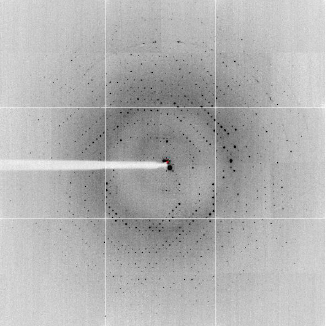
\includegraphics[width=\textwidth]{figures/introduction/intensityloss_kGydose.png}
                    \caption{Low dose $\sim kGy$ dataset.}
                    \label{fig:Intensity decay insulin diffraction image kGy}
            \end{subfigure}
            \quad
            \begin{subfigure}[b]{0.45\textwidth}
                    \centering
                    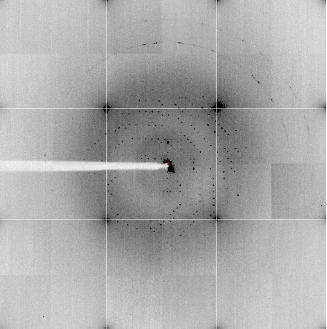
\includegraphics[width=\textwidth]{figures/introduction/intensityloss_30MGy.png}
                    \caption{High dose ($30\ MGy$) dataset.}
                    \label{fig:Intensity decay insulin diffraction image 30MGy}
            \end{subfigure}
            \\
            \begin{subfigure}[b]{0.45\textwidth}
                    \centering
                    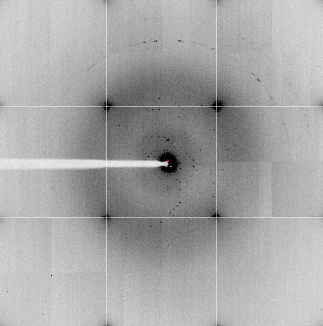
\includegraphics[width=\textwidth]{figures/introduction/intensityloss_60MGy.png}
                    \caption{Extremely high dose ($60\ MGy$) dataset.}
                    \label{fig:Intensity decay insulin diffraction image 60MGy}
            \end{subfigure}
            \caption{Intensity decay of reflections on diffraction images of cubic insulin collected at $100\ K$ with increasing radiation exposure. The intensity of reflections corresponding to high resolution information (spots closer to the edges of the images) decay faster than low resolution reflections.}
            \label{fig:Intensity decay insulin diffraction images}
        \end{figure}

        To observe appreciable changes in reciprocal space, radiation damage must be affecting the long range crystalline order of the of the crystal \cite{meents2010}.
        At room temperature, many more radical species are mobile and damage occurs much more quickly than at cryo-temperatures ($100\ K$) \cite{henderson1990cryo,weik2010temperature}.
        However, global radiation damage still occurs at cryo-temperatures and it has been proposed that this is due to hydrogen gas build up.
		This is because diffusion rates are smaller at lower temperatures.
		This build up of hydrogen exerts a disruptive force on the crystalline structure leading to the reduction in structural integrity \cite{meents2010}.

        The various symptoms or variants of them have been proposed as metrics to assess the extent of radiation damage as a function of the dose (Figure~\ref{fig:Radiation damage metrics}).
        An ideal metric would change reproducibly and monotonically with the increase in the dose.
        This rules out using the mosaicity as a suitable metric as it violates both of these criteria \cite{garman2010}.
        Unit cell volume expansion was once thought to be a suitable metric \cite{ravelli2002}, however it was determined later that it was not reliable because the expansion was not consistent amongst crystals of the same protein and the same size \cite{murray2002}.
        Three promising metrics that seem to adhere to the criteria (within a factor of 2) are: the decay R factor \cite{diederichs2006}, relative B factor \cite{kmetko2006} and the relative intensity \cite{owen2006}.

        \begin{figure}
            \centering
            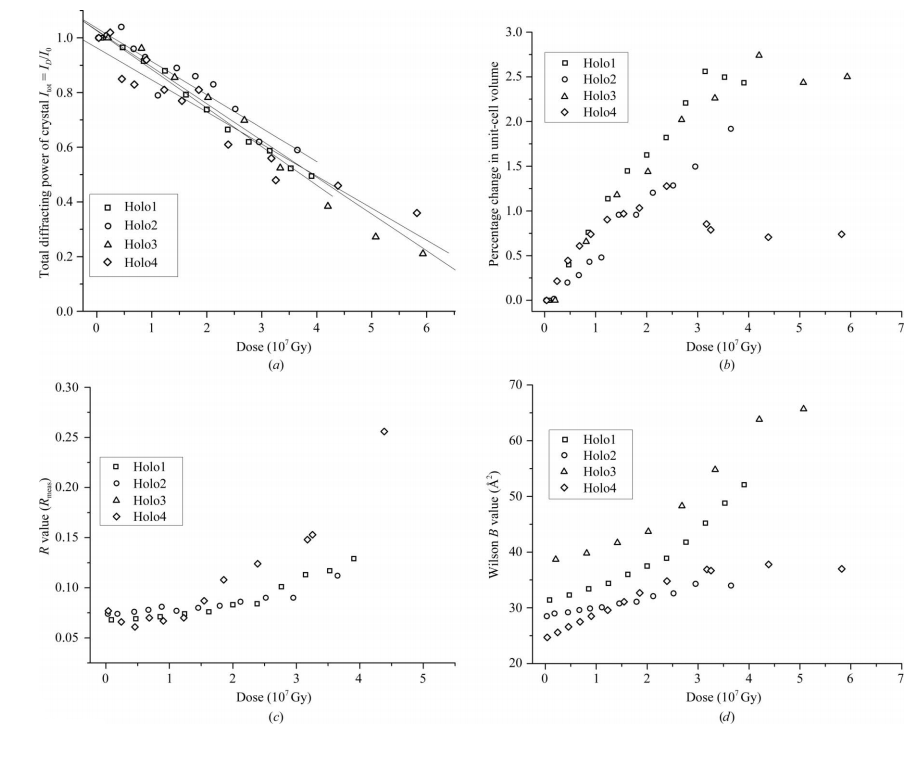
\includegraphics[width=1.0\textwidth]{figures/introduction/raddammetrics.png}
            \caption{Various global radiation damage metrics as a function of dose for four holoferritin crystals. Work performed by \cite{owen2006}, reproduced from \cite{garman2010}.}
            \label{fig:Radiation damage metrics}
        \end{figure}

        \subsubsection{Decay R factor}
        \label{subs:Decay R factor}
            The decay R factor, $R_d$ is decay metric that assesses the pairwise difference between symmetry related reflections on different images \cite{diederichs2006}.
            This results in a relatively smooth function against image number (used as a proxy for dose) that can be interpreted as follows: if $R_d$ stays constant for each image then no significant radiation damage has occurred, whereas if the $R_d$ increases then radiation damage is in progressing throughout the dataset.
            A desirable feature of this metric is that it can be used with a single dataset.
            Therefore radiation damage analysis can be performed on highly sensitive crystals that may only withstand enough dose for a single dataset.
			The problem is that it requires high multiplicity which is not always achievable. This metric is less commonly used in radiation damage studies than the other two.

        \subsubsection{Relative B factor}
        \label{subs:Relative B factor}
            The relative B factor, $B_{rel}$, is a metric that calculates the difference between the isotropic B factor for the initial dataset and a later dataset collected on the same crystal \cite{kmetko2006}.
            Various studies have shown that $B_{rel}$ increases linearly with dose \cite{kmetko2006,borek2007many,bourenkov2010optimization,leal2012}.
            Another closely related metric which is derived from $B_{rel}$ is the coefficient of sensitivity to absorbed dose, $s_{AD} = \Delta B_{rel} / \Delta D 8\pi^2$ where $\Delta B_{rel}$ and $\Delta D$ is the change in relative B factor and dose respectively. The advantage of $s_{AD}$ is that it is robust (to within a factor of 2) for protein crystals of differing molecular weights and solvent contents \cite{kmetko2006}.

        \subsubsection{Relative intensity}
        \label{subs:Relative intensity}
            The relative intensity is defined as $I_n/I_1$, where $I_n$ is the summed mean intensity of a complete data set $n$ (or equivalent sections of data) after a dose $D$, and $I_1$ is the mean intensity of the first data set \cite{garman2010}.
            This metric is desirable because it directly analyses the decay of the experimental data: the intensities. Furthermore it exhibits a linear dependence on the dose for a suitably low dose \cite{owen2006,zeldin2013dwd}.
            An experimental dose limit of $30\ MGy$ was established based on the observation that crystals of proteins with different compositions decay at the same rate at cryo-temperatures \cite{owen2006}.
            At this dose the relative intensity of the crystals had decayed to 70\% of their initial value, at which point it is regarded that the structural information that can be determined from the sample has been significantly compromised \cite{owen2006,blundell1976protein}.

    \subsection{Manifestations of damage: Specific damage}
    \label{sub:Manifestations of damage: Specific damage}
        In contrast to global radiation damage, specific radiation damage is classified as damage that is observed in real space in the electron density maps and occurs up to $\approx 60$ times faster \cite{holton2009}.
        It is characterised by what appear to be specific chemical changes to the molecule and occurs in a reproducible order \cite{ravelli2000,weik2000,gerstel2015identifying}:
        \begin{enumerate}
            \item Metallo-centres are reduced at doses as low as $45\ kGy$ \cite{owen2011revealing}.
            \item Elongation and breakage of disulphide bonds \cite{burmeister2000structural,ravelli2000}.
            \item Decarboxylation of glutamate and aspartate residues \cite{burmeister2000structural,weik2000,ravelli2000}.
            \item The $S^{\delta}-C^{\epsilon}$ bond of methionine residues is cleaved \cite{burmeister2000structural}.
            \item Covalent metal bonds are cleaved \cite{ramagopal2005radiation}.
        \end{enumerate}
        Dehydroxylation of tyrosine residues have also been observed \cite{burmeister2000structural}, but the physical basis and the evidence of this being a general symptom of specific radiation damage is contentious (Charlie Bury and Elspeth Garman, personal communication).

		Due to the fact that specific damage changes structural information, it can lead to incorrect biological interpretation from structures.
		Metrics to assess the progression of specific damage also exist but are not always described as a function of dose.

        \subsubsection{Peaks in Fourier difference maps}
        \label{subs:Peaks in Fourier difference maps}
            Fourier difference maps, $F_n - F_1$, are electron density maps where the amplitudes of the first dataset $F_1$ are subtracted from the amplitudes of a later dataset $F_n$.
			Negative values correspond to areas where electron density has been lost as the experiment progressed.
			Sometimes this can be due to noise in the data, but significantly high values (difference peaks) that are coincident with the structural model from the first dataset suggest specific structural damage has occurred.
			In most studies, this sort of analysis is done via manual inspection of the electron density map \cite{burmeister2000structural,weik2000,ravelli2000}.
			However work is being done towards automating this analysis and developing new metrics to better characterise the level of specific damage \cite{bury2015radiation}.

        \subsubsection{Atomic B-factors}
        \label{subs:Atomic B-factors}
            Atomic B-factors (also referred to as atomic displacement parameters) describe the level of dynamic disorder of atoms, with each atom having its own B-factor.
			Generally this value increases as radiation damage progresses and the level of disorder of the structure increases.
			In practice the B-factor is also substantially influenced by other factors such as static disorder (occupancy), errors in model building and the packing density of the atom \cite{gerstel2015identifying}.
			This means that atoms with higher B-factors may not necessarily be more damaged than atoms with a smaller B-factor.

        \subsubsection{B damage}
        \label{subs:B damage}
            B damage, $B_{damage}$, is a metric that aims to deconvolute the dependence of the atomic B factor on it's packing density.
			It is defined as the ratio of an atom's B-factor and the average B-factor of atoms that have a similar packing density environment \cite{gerstel2015identifying}.
			This is a normalised metric, therefore atoms that show damage will have $B_{damage}$ values significantly greater than 1.

        Analysis of PDB structures with $B_{damage}$ showed a positive correlation between radiation damage and solvent accessibility \cite{gerstel2015identifying}, in agreement with statements made in \cite{sygusch1988}.
		However other studies have claimed otherwise \cite{coquelle2007activity,homer2011energy} demonstrating the lack of consensus of metrics and conclusions in radiation damage studies.

    \subsection{Experimental methods for dealing with radiation damage}
    \label{sub:Experimental methods for dealing with radiation damage}
        Due to the challenge presented by radiation damage in MX to achieve successful structure determination, various parameters of the experiment have been varied in an attempt to mitigate its effects.

        \subsubsection{Temperature}
        \label{subs:Temperature}
            It has been known for decades that diffraction experiments carried out at cryo-temperatures ($100\ K$) improves the lifetime of biological samples \cite{henderson1990cryo,brooks2015nobel} by around $\sim 25 - 110$ times over room temperature (RT) experiments \cite{south2007}.
            Cryo-cooling requires careful protection of the sample to prevent freezing, because ice also exhibits a crystalline structure that will too diffract coherently in the MX experiment.
            Cryo-protection techniques have been developed since the late 1980s \cite{garman1997macromolecular,hope1988cryocrystallography,teng1990mounting} and cryo-crystallography is now more routine than RT experiments \cite{garman2014}.
            The main problem with cryo-cooling a crystal is that it can decrease the crystalline order of the crystal \cite{nave2005} although this is not always the case \cite{garman1999cool}.

            There is evidence to suggest that using temperatures below $100\ K$ may further improve the lifetime of crystals and the data quality \cite{meents2010,teng2002}.
            However, whether the benefits of cooling to temperatures of $40\ K$ or below are significant enough to warrant the costs required to achieve those temperatures routinely is still not obvious \cite{weik2010temperature}.

        \subsubsection{Dose rate}
        \label{subs:Dose rate}
            Damage processes occur over a finite time period and this has been exploited by increasing the rate at which the dose is deposited in the crystal (dose rate) in an attempt to outrun radiation damage.
			At cryo-temperatures dose rate effects have been shown to improve crystal lifetimes by up to 10\% \cite{owen2006} although some report that there is no effect at all \cite{sliz2003}.
			At RT the evidence that there is a dose rate dependence seems is quite convincing \cite{south2007,owen2012,owen2014}.
			With the increasingly popularity of \textit{in situ} data collection \cite{axford2015structure,axford2012situ}, particularly for protein crystals that are not amenable to cryo-cooling, high dose rate experiments are likely to become even more routine.

            Serial femtosecond crystallography (SFX) at XFELs use incredibly fast X-ray pulses (as little as $5 fs$ \cite{boutet2012high}) to probe protein crystals to obtain ``diffraction before destruction" \cite{chapman2014diffraction}.
			Although experimental data have now shown indications that radiation damage is still visible at XFELs if the pulse length is too long \cite{nass2015indications}.
			SFX at XFELs are still in their infancy but progress is continuously being made and is a promising field for the development of structural biology \cite{garman2014,brooks2015nobel}.


        \subsubsection{Scavengers}
        \label{subs:Scavengers}
            Scavengers are small molecules introduced to the crystal to mitigate the effects of secondary damage by ``soaking" up radicals.
			At present, evidence of the efficacy of scavengers is contradictory.
			For example the studies presented in \cite{barker2009room,kmetko2011can} are conflicting in their evidence as to whether scavengers have any effect on global radiation damage metrics.
			It is worth noting that the studies used different global radiation damage metrics ($I_n/I_1$ improved with use of scavengers, whereas $B_{rel}$ did not) to come to their conclusions.
			The effect of scavengers to protect against specific radiation damage is more promising \cite{southworth2007radioprotectant}.
			A comprehensive summary of all scavenger literature to date is provided in \cite{allan2012}.

    \subsection{Modelling intensity decay}
    \label{sub:Modelling intensity decay}
        Structure factor amplitudes are derived from the integrated intensity measurements from the experimental data.
        Therefore accurate intensity values are required to obtain reliable structural information.
		The problem is that the intensity measurements are affected by several systematic factors \cite{evans2005}.
		In particular, global radiation damage of the sample can be a significant factor contributing to the overall intensity variation.
		For this reason attempts to correct for this effect have been proposed and implemented during data processing.

        The first systematic study of radiation damage was carried out on crystals of sperm whale myoglobin in 1962 by Blake and Phillips \cite{blake1962}.
        In this study they determined that radiation damage progression is proportional to the absorbed dose and predicted that specific damage was occurring without knowledge of the sequence of the molecule.
        Repeated intensity measurements of a subset of reflections along the $h0l$ zone were taken with increasing X-ray exposure.
        \textcolor{red}{
            \begin{myenumerate}
                \item \hypertarget{todo:checkrefzone}{\textbf{TODO:} Check that the reflection zone is $h0l$, not $010$ as written in \cite{south2007}. Elspeth: do you have the Blake and Phillips paper to hand?}
            \end{myenumerate}
        }
        It was noted that there was a general decrease in the intensity values with reflections corresponding to higher resolution decaying quickest.
        If the variation was due solely to thermal disorder then the intensity decay was expected to obey the form
        \begin{equation}
            I = I_0 \exp\left(-\f{B \sin^2(\theta)}{\lambda^2} \right),
        \end{equation}
        where $I$ is the experimentally measured intensity, $I_0$ is the initial intensity, $B$ is a measure of the disorder, $\theta$ is the diffraction angle and $\lambda$ is the wavelength of the incident beam.
        However this form did not explain the observation that the intensity flattened out at high $\theta$ angles.
        So a compartmental model of the crystal was proposed. The three states that were used to describe the evolution of the crystal damage were
        \begin{enumerate}
            \item $A_1$ - an undamaged fraction of the crystal which contributes to diffraction at all angles.
            \item $A_2$ - a highly disordered fraction that only contributes to diffraction at low angles.
            \item $A_3 = 1 - (A_1 + A_2)$ - an amorphous fraction that no longer diffracts coherently.
        \end{enumerate}
        These compartments were suggested to contribute to the diffracted intensity, $I$, at time $t$ as
        \begin{equation}
            \f{I(t)}{I(0)} = A_1(t) + A_2(t) \exp\left(-\f{B\sin^2(\theta)}{\lambda^2} \right).
            \label{eq:Blake and Phillips Radiation Damage Model}
        \end{equation}
        To explain the crystal compartment dynamics (i.e. how the crystal transitions between damaged, highly disordered and amorphous states) it was assumed that radiation damage effects are irreversible. The transitions are described according to Figure~\ref{fig:Crystal Compartments Blake and Phillips} where $k_1, k_2$ and $k_3$ are rate constants to be determined.
        \begin{figure}[H]
            \centering
            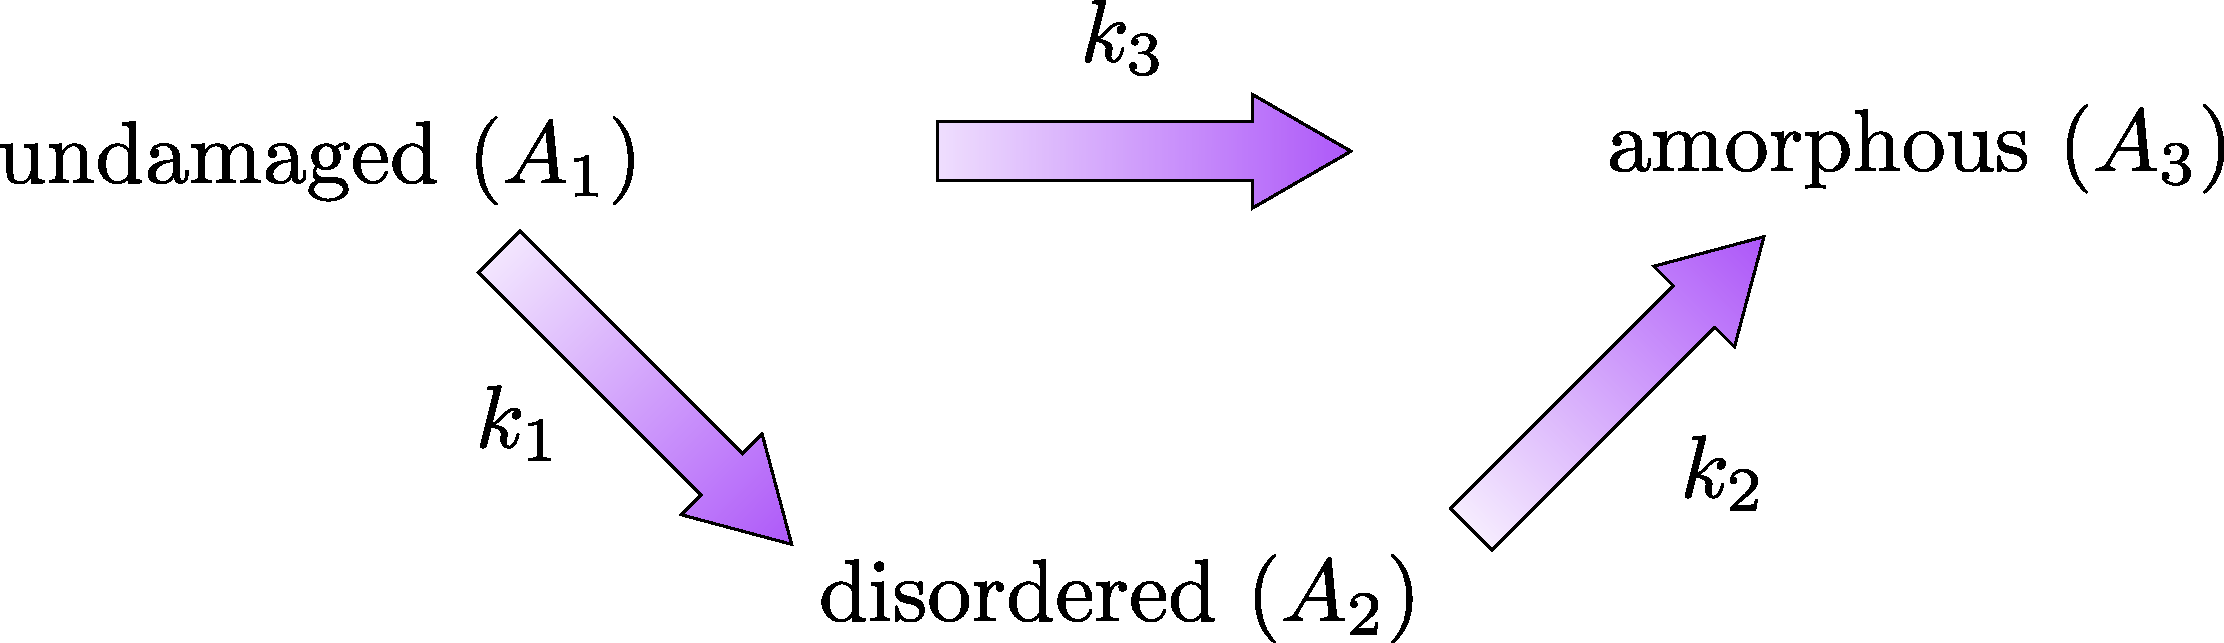
\includegraphics[width=0.8\textwidth]{figures/introduction/crystalcompartments_BP.pdf}
            \caption{Transition dynamics of the compartments in the Blake and Phillips model. Note here that the states are irreversible and it is possible to transition directly from the undamaged fraction to the amorphous fraction.}
            \label{fig:Crystal Compartments Blake and Phillips}
        \end{figure}
        The intensity measurements corrected with equation \ref{eq:Blake and Phillips Radiation Damage Model} generally agreed well with the measurements from the relatively undamaged crystal.

        The Blake and Phillips model was also used to correct for radiation damage for a study on crystals of lamprey haemoglobin \cite{hendrickson1973}. In this study, 150 reflections were observed to determine the change in intensity as a function of the dose. The data they recorded agreed well with the model of Blake and Phillips.

        In 1976, Fletterick \textit{et al.} proposed a modification to the Blake and Phillips model for their study on  glycogen phosphorylase a crystals \cite{fletterick1976low}.
        The modification disallowed a direct transition from the undamaged state to the amorphous state (i.e. $k_3 = 0$ in Figure~\ref{fig:Crystal Compartments Blake and Phillips}). This gives the sequential transition model
        \begin{equation}
            A_1 \xrightarrow{k_1} A_2 \xrightarrow{k_2} A_3.
        \end{equation}
        In 1976, Hendrickson studied all possible transitions from the Blake and Phillips model (Figure~\ref{fig:Crystal Compartments Blake and Phillips}) assuming irreversible transition states \cite{hendrickson1976}.
        This included $k_2 = k_3$ \cite{hendrickson1973}, $k_1 = k_2$ and $k_3 = 0$, $k_3 = 0$ \cite{fletterick1976low}, $k_1 + k_3 = k_2$ and the arbitrary time-dependence model.
        These models were fitted to the data from the Blake and Phillips myoglobin study \cite{blake1962}.
        It was concluded that all models explain the data well for moderate dose values ($\approx$ 26\% damage), but none explain radiation damage at high doses very well ($\approx$ 72\% damage).
        The general model resulted in refined $k_3$ values that were very close to zero, and the model with $k_3 = 0$ consistently resulted in the best fit to the data at higher dose values.
        This suggests that the radiation damage process is sequential.

		In 1988 Sygusch and Allaire proposed an extension to the Fletterick \textit{et al.} model.
        They suggested that a fourth fraction, $A'_1$, that has only suffered small perturbations of surface residues and disulphide bonds, still has the capability of contributing to diffraction that occurs at all angles \cite{sygusch1988}.
        This is because these surface perturbations are caused before any significant changes in molecular conformation.
        The resulting sequential model is expressed as
        \begin{equation}
            A_1 \xrightarrow{k_1} A'_1 \xrightarrow{k_1} A_2 \xrightarrow{k_2} A_3.
        \end{equation}
        This model was fitted with data collected on crystals of rabbit skeletal muscle aldolase. The authors show that the proposed model provides a very good fit for radiation damage even at high doses.

        In 2009 James Holton proposed an resolution dependent model of intensity decay for a reflection \cite{holton2009}. This model considers the absorbed dose within the crystal and describes the intensity decay of a reflection, $I$, as
        \begin{equation}
            I = I_0 \exp \left(-\ln(2)\f{D}{Hd}\right)
        \end{equation}
        where $I_0$ is the intensity at zero dose, $D$ is the absorbed dose in $MGy$, $d$ is the resolution of the reflection in \AA\ corresponding to the distance between successive Bragg planes, and $H$ is the Howells \textit{et al.} criterion which proposed a resolution dependent dose limit of $10\ MGy$ per \AA\ \cite{howells2009}.
		This model was shown to produce results in agreement with those from \cite{owen2006,kmetko2006} when tested with their data.

        In 2012 Leal \textit{et al.} modified a traditional scaling model to account for radiation damage \cite{leal2012}. The scaling model defined as
        \begin{equation}
            J(D,\bs{h}) = J(h_d) \times K(D) \times \exp\left( -B(D) h_d^2/2\right)
			\label{eq:Scaling Model Leal 2012}
        \end{equation}
        where $J(D,\bs{h})$ is the expected intensity of a given reflection with Miller indices $\bs{h} = hkl$ after the crystal has absorbed a dose $D$, and $J(h_d)$ is the expected reflection intensity at reciprocal distance $h_d = |\bs{h}| = 1/d$ from the origin in the absence of any radiation damage.
		$K(D)$ and $B(D)$ are the scale and B-factors respectively and both are dependent on the absorbed dose.
		The authors assumed a linear model of B-factor increase given by
		\begin{equation}
			B(D) = B_0 + D \beta,
            \label{eq:Linear B factor dependence}
		\end{equation}
		where $B_0$ and $\beta$ are empirical constants to be determined.
		The authors empirically deduced the functional form of the scale factor, $K$ as
		\begin{equation}
			K(D) = C \exp\left(-\gamma^2 D^2\right),
            \label{eq:Gaussian Scale factor dependence}
		\end{equation}
		where $C$ and $\gamma$ are empirical constants to be determined.
        The $D^2$ in equation \ref{eq:Gaussian Scale factor dependence} means that the model proposed by Leal \textit{et al.} is essentially Gaussian decay behaviour.
		This model was shown to agree well with the overall intensity decay for data collected on 15 different crystals at RT to a relative intensity down to 60\% of the original value.

		Despite the differences between these models, they each rely on an accurate calculation of the dose absorbed within a crystal.
		Of particular note, the models proposed by Sygusch and Allaire and Leal \textit{et al.} allow for a delayed intensity decay.
		For the Leal \textit{et al.} model, this behaviour follows from the Gaussian form of the equation.
		The Sygusch and Allaire model was shown to exhibit this behaviour by fitting the model to experimental data \cite{owen2014}.

		Current scaling methods employ a scaling equation in the same form as equation \ref{eq:Scaling Model Leal 2012} to place multiple datasets on the same scale \cite{kabsch2010integration}.
        However the functional forms of the scale and B-factors are not necessarily assumed to take the forms given by equations \ref{eq:Linear B factor dependence} and \ref{eq:Gaussian Scale factor dependence}.
		The scaling of intensities on images within a dataset also takes a form very similar to equation \ref{eq:Scaling Model Leal 2012}. Take, for example the scaling model used in AIMLESS:
        \begin{equation}
            g = g_1(\varphi) \times g_2(\bs{s}_2) \times \exp \left(\f{-2B(\varphi)\sin^2(\theta)}{\lambda^2} \right),
        \end{equation}
		where $g$ is the factor that puts the intensity on an internally consistent scale with the other images in the dataset, $g_1$ and $g_2$ are scaling factors, $\varphi$ is the crystal rotation angle which is used as a proxy for the primary beam direction and the dose and $\bs{s}_2$ is the secondary beam direction \cite{evans2013}.
		The crystal rotation angle, $\varphi$, is used as a proxy for dose because the dose is not routinely calculated in MX experiments. It is noted by Evans and Murshudov that the B-factor correction in this model is largely an average correction.

		Many studies, including the first by Blake and Phillips, found that the decay of individual reflection intensities is not necessarily monotonic \cite{blake1962,hendrickson1973,hendrickson1976}.
		As well as diffraction being anisotropic \cite{abrahams1987anisotropy}, some reflection reflections also increase in intensity with increasing dose \cite{abrahams1973}.

		Therefore the average radiation damage correction will not account for the specific changes that are known to occur.
		Diederichs \textit{et al.} used a linear function to correct individual reflection intensities up to a dose of $10\ MGy$ and showed that this reflection specific correction could improve results of SAD phasing \cite{diederichs2003}.
		Diederichs later used quadratic and exponential functions to correct individual reflection intensities \cite{diederichs2006}.
		It was concluded that the quadratic model suffers from the problem that it requires two parameters to be fitted for each reflection and it is not suitable when the unit cell expands because the Fourier transform of the molecule is no longer consistent between observations of the same reflection.
		The linear model suffers from the problem that the fitted parameter doesn't have a physical interpretation and the correction can result in negative extrapolated intensities.
		The exponential model has the advantage that it only results in positive values but again it lacks physical interpretation.

		Despite some of the drawbacks, these specific correction models have shown some promise, but as of yet these types of corrections are not standard. This is because they are not necessarily straight forward to implement and they don't always seem to improve the data quality (Phil Evans, personal communication).
